% Options for packages loaded elsewhere
\PassOptionsToPackage{unicode}{hyperref}
\PassOptionsToPackage{hyphens}{url}
%
\documentclass[
  ignorenonframetext,
  aspectratio=169]{beamer}
\title{Measures of central tendency and frequency distribution}
\author{Deependra Dhakal}
\date{}
\institute{Assistant Professor \and Agriculture and Forestry
University \and \url{https://rookie.rbind.io}}

\usepackage{pgfpages}
\setbeamertemplate{caption}[numbered]
\setbeamertemplate{caption label separator}{: }
\setbeamercolor{caption name}{fg=normal text.fg}
\beamertemplatenavigationsymbolsempty
% Prevent slide breaks in the middle of a paragraph
\widowpenalties 1 10000
\raggedbottom
\setbeamertemplate{part page}{
  \centering
  \begin{beamercolorbox}[sep=16pt,center]{part title}
    \usebeamerfont{part title}\insertpart\par
  \end{beamercolorbox}
}
\setbeamertemplate{section page}{
  \centering
  \begin{beamercolorbox}[sep=12pt,center]{part title}
    \usebeamerfont{section title}\insertsection\par
  \end{beamercolorbox}
}
\setbeamertemplate{subsection page}{
  \centering
  \begin{beamercolorbox}[sep=8pt,center]{part title}
    \usebeamerfont{subsection title}\insertsubsection\par
  \end{beamercolorbox}
}
\AtBeginPart{
  \frame{\partpage}
}
\AtBeginSection{
  \ifbibliography
  \else
    \frame{\sectionpage}
  \fi
}
\AtBeginSubsection{
  \frame{\subsectionpage}
}
\usepackage{amsmath,amssymb}
\usepackage{lmodern}
\usepackage{iftex}
\ifPDFTeX
  \usepackage[T1]{fontenc}
  \usepackage[utf8]{inputenc}
  \usepackage{textcomp} % provide euro and other symbols
\else % if luatex or xetex
  \usepackage{unicode-math}
  \defaultfontfeatures{Scale=MatchLowercase}
  \defaultfontfeatures[\rmfamily]{Ligatures=TeX,Scale=1}
\fi
\usetheme[]{Frankfurt}
\usecolortheme{beaver}
% Use upquote if available, for straight quotes in verbatim environments
\IfFileExists{upquote.sty}{\usepackage{upquote}}{}
\IfFileExists{microtype.sty}{% use microtype if available
  \usepackage[]{microtype}
  \UseMicrotypeSet[protrusion]{basicmath} % disable protrusion for tt fonts
}{}
\makeatletter
\@ifundefined{KOMAClassName}{% if non-KOMA class
  \IfFileExists{parskip.sty}{%
    \usepackage{parskip}
  }{% else
    \setlength{\parindent}{0pt}
    \setlength{\parskip}{6pt plus 2pt minus 1pt}}
}{% if KOMA class
  \KOMAoptions{parskip=half}}
\makeatother
\usepackage{xcolor}
\IfFileExists{xurl.sty}{\usepackage{xurl}}{} % add URL line breaks if available
\IfFileExists{bookmark.sty}{\usepackage{bookmark}}{\usepackage{hyperref}}
\hypersetup{
  pdftitle={Measures of central tendency and frequency distribution},
  pdfauthor={Deependra Dhakal},
  hidelinks,
  pdfcreator={LaTeX via pandoc}}
\urlstyle{same} % disable monospaced font for URLs
\newif\ifbibliography
\setlength{\emergencystretch}{3em} % prevent overfull lines
\providecommand{\tightlist}{%
  \setlength{\itemsep}{0pt}\setlength{\parskip}{0pt}}
\setcounter{secnumdepth}{-\maxdimen} % remove section numbering
\usepackage{setspace}
\usepackage{wasysym}
\usepackage{fontenc}
\usepackage{booktabs,siunitx}
\usepackage{longtable}
\usepackage{array}
\usepackage{multirow}
\usepackage{wrapfig}
\usepackage{float}
\usepackage{colortbl}
\usepackage{pdflscape}
\usepackage{tabu}
\usepackage{threeparttable}
\usepackage{threeparttablex}
\usepackage[normalem]{ulem}
\usepackage{makecell}
\usepackage{xcolor}
\usepackage{tikz} % required for image opacity change
\usepackage[absolute,overlay]{textpos} % for text formatting
\usepackage[skip=0.3\baselineskip]{caption}
% \usepackage{newtxtext,newtxmath}% better than txfonts   

% this font option is amenable for beamer
\setbeamerfont{caption}{size=\tiny}
\singlespacing

\sisetup{per-mode=symbol}

\newcommand\Myperm[2][^n]{\prescript{#1\mkern-2.5mu}{}P_{#2}}
\newcommand\Mycomb[2][^n]{\prescript{#1\mkern-0.5mu}{}C_{#2}}

% \setcounter{totalnumber}{50}
% \setcounter{topnumber}{50}
% \setcounter{bottomnumber}{50}
% \setlist[itemize,1]{leftmargin=2pt,itemindent=2pt}
% \setlist[itemize,2]{leftmargin=6pt,itemindent=2pt}
% \def\labelitemi{$\bullet$}
% \def\labelitemii{$\diamond$}
% \def\labelitemiii{\textbullet}
\captionsetup[table]{skip=0pt}
\captionsetup[table]{belowskip=-2pt}
\setbeamerfont{caption}{size=\tiny}
\setbeamertemplate{footline}[page number]
\AtBeginSection{}
\AtBeginSubsection{}
\ifLuaTeX
  \usepackage{selnolig}  % disable illegal ligatures
\fi

\begin{document}
\frame{\titlepage}

\begin{frame}[allowframebreaks]
  \tableofcontents[hideallsubsections]
\end{frame}
\hypertarget{measures-of-central-tendency}{%
\section{Measures of central
tendency}\label{measures-of-central-tendency}}

\begin{frame}{}
\protect\hypertarget{section}{}
\small

\begin{itemize}
\tightlist
\item
  \textbf{Descriptive statistics} are statistics that describe a set of
  data.
\item
  For quantitative data

  \begin{itemize}
  \tightlist
  \item
    They show a tendency to concentrate at certain values, usually
    somewhere in centre of the distribution. Measures of this tendency
    are called measures of central tendency or averages.
  \item
    The data vary about a measure of central tendency and these measures
    of deviation are called measures of \emph{variation} or
    \emph{dispersion}.
  \item
    The data in a frequency distribution may fall into symmetrical or
    asymmetrical patterns. The measures of the direction and degree of
    asymmetry are called measures of \emph{skewness}.
  \item
    Polygons of frequency distributions exhibit flatness or peakedness
    of frequency curves. The measures of peakedness or flatness of the
    frequency curves are called measures of \emph{kurtosis}.
  \end{itemize}
\item
  For numerical data, the frequency distribution can usefully be
  supplemented by a few numerical measures.
\item
  For categorical data, the frequency distribution provides a concise
  and complete summary of a sample.
\item
  Measures of the ``center'' or ``typical value'' of the data can be
  defined in several ways.
\end{itemize}
\end{frame}

\begin{frame}{}
\protect\hypertarget{section-1}{}
\footnotesize

\begin{itemize}
\tightlist
\item
  A book-keeper sold following units of the same book during 20
  consecutive days. How can we describe the sales of the book ?
\end{itemize}

\[
12, 0, 5, 13, 0, 0, 5, 10, 5, 1, 5, 6, 7, 5, 7, 8, 10, 5, 11,14
\]

\begin{itemize}
\tightlist
\item
  arrange in order
\end{itemize}

\[
0, 0, 0, 1, 5, 5, 5, 5, 5, 5, 6 , 7, 7, 8, 10, 10, 11, 12, 13, 14
\]

\begin{itemize}
\tightlist
\item
  Mode is most frequently occuring number
\item
  Median is value that divides data in half
\item
  Mean

  \begin{itemize}
  \tightlist
  \item
    sum of all observations divided by number of observations
  \end{itemize}
\end{itemize}

\[
\small
\frac{12 + 0 + 5 + 13 + 0 + 0 + 5 + 10 + 5 + 1 + 5 + 6 + 7 + 5 + 7 + 8 + 10 + 5 + 11 +14}{20}
\]
\end{frame}

\begin{frame}{Arithmetic mean}
\protect\hypertarget{arithmetic-mean}{}
\begin{itemize}
\tightlist
\item
  The mean (sample mean) of a sample is the sum of the observations
  divided by the number of observations.
\end{itemize}

\[
\bar{y} = \frac{\sum_{i=1}^n{y_i}}{n}
\]

\begin{itemize}
\tightlist
\item
  where:

  \begin{itemize}
  \tightlist
  \item
    \(y_i\)'s are the observations in the sample and n is the sample
    size (that is, the number of \(y_i\)'s)
  \end{itemize}
\end{itemize}
\end{frame}

\begin{frame}{Mean of grouped data}
\protect\hypertarget{mean-of-grouped-data}{}
\small

\begin{columns}[T, onlytextwidth]
\column{0.4\textwidth}

$$
\begin{aligned}
\bar{y} = \frac{\sum_{k= 1}^r f_k y_k}{\sum_{k= 1}^r f_k}
\end{aligned}
$$

Where:

$f_k$ and $y_k$ are the frequency and numerical value of the $k^{\text{th}}$ item in the collection. 

$y_k$ also refers to the midpoint value of the $k^{\text{th}}$ class in a grouped numeric data having fixed class intervals.

\column{0.6\textwidth}

(Statistics for the Life Sciences, 2016) An agronomist counted the number of leaves on each of 150 tobacco plants of the same strain (Havana). The results are shown in Table \ref{tab:num-leaves-tobacco}.

\begin{table}

\caption{\label{tab:num-leaves-tobacco}Number of leaves on tobacco plants}
\centering
\fontsize{7}{9}\selectfont
\begin{tabular}[t]{rr}
\toprule
Number of leaves & Frequency (number of plants)\\
\midrule
17 & 3\\
18 & 22\\
19 & 44\\
20 & 42\\
21 & 22\\
\addlinespace
22 & 10\\
23 & 6\\
24 & 1\\
\bottomrule
\end{tabular}
\end{table}

For the data given above,

$\bar{y}$ = 19.78.

\end{columns}
\end{frame}

\begin{frame}{Median}
\protect\hypertarget{median}{}
\begin{itemize}
\tightlist
\item
  The sample median is the value that most nearly lies in the middle of
  the sample -- the data value that splits the ordered data into two
  equal halves.
\item
  Requires construction of ordered array
\item
  Median is denoted by \(\tilde{y}\)
\end{itemize}
\end{frame}

\begin{frame}{Median of grouped data}
\protect\hypertarget{median-of-grouped-data}{}
\begin{columns}[T, onlytextwidth]
\column{0.5\textwidth}
\footnotesize
Steps

\begin{itemize}
\scriptsize
\item Construct the cumulative frequency distribution
\item Decide the class that contain the median. \alert{Class median} is the first class with the value of cumulative frequency equal at least $\frac{n}{2}$
\item Median is given by following formula:
\end{itemize}

$$
\small
\text{Median} = L_m + \left(  \frac{\frac{n}{2} - F}{f_m} \right)
$$

Where:

\begin{itemize}
\scriptsize
\item $n$ = total frequency
\item $F$ = cumulative frequency \alert{before} class median
\item $f_m$ = frequency of the class median
\item $i$ = class width
\item $L_m$ = lower boundary of the class median
\end{itemize}

\column{0.5\textwidth}

\footnotesize
Based on the grouped data below, find the medium.

\begin{table}

\caption{\label{tab:grouped-data-example}Frequency distribution of time to travel to work also showing cumulative class interval frequencies for successive classes}
\centering
\fontsize{7}{9}\selectfont
\begin{tabular}[t]{>{\raggedright\arraybackslash}p{8em}>{\raggedright\arraybackslash}p{6em}>{\raggedright\arraybackslash}p{7em}}
\toprule
Time to travel to work & Frequency & Cumulative frequency\\
\midrule
1 - 10 & 8 & 8\\
11 - 20 & 14 & 22\\
21 - 30 & 12 & 34\\
31 - 40 & 9 & 43\\
41 - 50 & 7 & 50\\
\bottomrule
\end{tabular}
\end{table}

\footnotesize
$\frac{n}{2}$ = $\frac{50}{2}$ = 25 $\longrightarrow$ class median in the $3^{\text{rd}}$ class,

So, $F = 22$, $f_m = 12$, $L_m = 20.5$ and $i = 10$.

$\therefore$ Median = $21.5 + \left(\frac{25-22}{12}\right)\times 10$ = 24.

Thus, 25 persons take less than 24 minutes to travel to work and another 25 persons take more than 24 minutes to travel to work.

\end{columns}
\end{frame}

\begin{frame}{Interquartile range of grouped data}
\protect\hypertarget{interquartile-range-of-grouped-data}{}
\begin{itemize}
\tightlist
\item
  The above expression for Median can be modified so that we can get the
  \(Q_1\) and \(Q_3\) as follows:
\end{itemize}

\begin{columns}[T,onlytextwidth]
\column{0.5\textwidth}

$$
\small
\mathrm{Q_1} = L_{Q_1} + \left(  \frac{\frac{n}{4} - F}{f_{Q_1}} \right)
$$
\column{0.5\textwidth}

$$
\small
\mathrm{Q_3} = L_{Q_3} + \left(  \frac{\frac{3n}{4} - F}{f_{Q_3}} \right)
$$

\end{columns}

Now,

\begin{block}{Interquartile range (IQR)}
$IQR = \mathrm{Q_3} - \mathrm{Q_1}$
\end{block}
\end{frame}

\begin{frame}{Mode}
\protect\hypertarget{mode}{}
\begin{itemize}
\tightlist
\item
  Mode is the value that has the highest frequency in a data set.
\item
  For grouped data, class mode (or modal class) is the class with the
  highest frequency.
\item
  Following formula gives the mode of the given set of grouped data:
\end{itemize}

\[
\text{Mode} = L_{mo} + \left( \frac{\Delta_1}{\Delta_1 + \Delta_2} \right)\times i
\]

\begin{itemize}
\tightlist
\item
  Where:

  \begin{itemize}
  \tightlist
  \item
    \(i\) is the class width
  \item
    \(\Delta_1\) is the difference between the frequency of class mode
    and the frequency of the class after the class mode
  \item
    \(\Delta_2\) is the difference between the frequency of class mode
    and the frequency of the class before the class mode
  \item
    \(L_{mo}\) is the lower boundary of class mode
  \end{itemize}
\end{itemize}
\end{frame}

\begin{frame}{Numerical example}
\protect\hypertarget{numerical-example}{}
\footnotesize

The number of days that children were missing from school due to
sickness in on year was recorded. Estimate the mean, medium and the
modal class.

\begin{table}
\centering\begingroup\fontsize{7}{9}\selectfont

\begin{tabular}{>{\raggedright\arraybackslash}p{8em}>{\raggedright\arraybackslash}p{6em}>{\raggedright\arraybackslash}p{6em}>{\raggedright\arraybackslash}p{5em}>{\raggedright\arraybackslash}p{5em}}
\toprule
Number of days off sick & Frequency ($f_k$) & Mid-point ($y_k$) & Cumulative frequency & $f_k\times y_k$\\
\midrule
1-5 & 12 & 3 & 12 & 36\\
6-10 & 11 & 8 & 23 & 88\\
11-15 & 10 & 13 & 33 & 130\\
16-20 & 4 & 18 & 37 & 72\\
21-25 & 3 & 23 & 40 & 69\\
\bottomrule
\end{tabular}
\endgroup{}
\end{table}

Mean = \(\frac{395}{40}\) = 9.925 days.

As there are 40 pupils, we need to consider the mean of the 20th and
21st values. These both lie in the 6-10 class interval (which is really
the 5.5-10.5 class).

As there are 12 values in the first class interval, the medium is found
by considering the 8th and 9th values of the second interval.

As there are 11 values in the second interval, the median is estimated
as being \(\frac{8.5}{11}\) of the way along the second interval.

But the length of the second interval is 10.5-5.5=5, so the median is
estimated by \(\frac{8.5}{11}\times 5 = 3.86\) from the start of this
interval. Therefore the median is estimated as: \(5.5 + 3.86 = 9.36\)
\end{frame}

\begin{frame}{Use case: library books}
\protect\hypertarget{use-case-library-books}{}
\begin{itemize}
\tightlist
\item
  Students borrow and return books from a university library regularly
\end{itemize}

\[
14, 13, 12, 11, 17, 20, 14, 16, 12, 12, 11, 9, 18, 21
\]

\begin{itemize}
\tightlist
\item
  One student borrows a book and forgets to return it
\item
  They re-discover the book 1 year later when moving out of the student
  accommodation and decide to return the book
\end{itemize}

\[
14, 13, 12, 11, 17, 20, 14, 16, 12, 12, 11, 9, 18, 21, 365
\]

\begin{itemize}
\tightlist
\item
  What do you think will happen to the mean and median of a data set on
  \textbf{borrowing periods}?
\end{itemize}
\end{frame}

\begin{frame}{}
\protect\hypertarget{section-2}{}
\begin{columns}[T, onlytextwidth]
\column{0.6\textwidth}

"A statistician drowned while crossing a river that was on average six inches deep"

\column{0.4\textwidth}


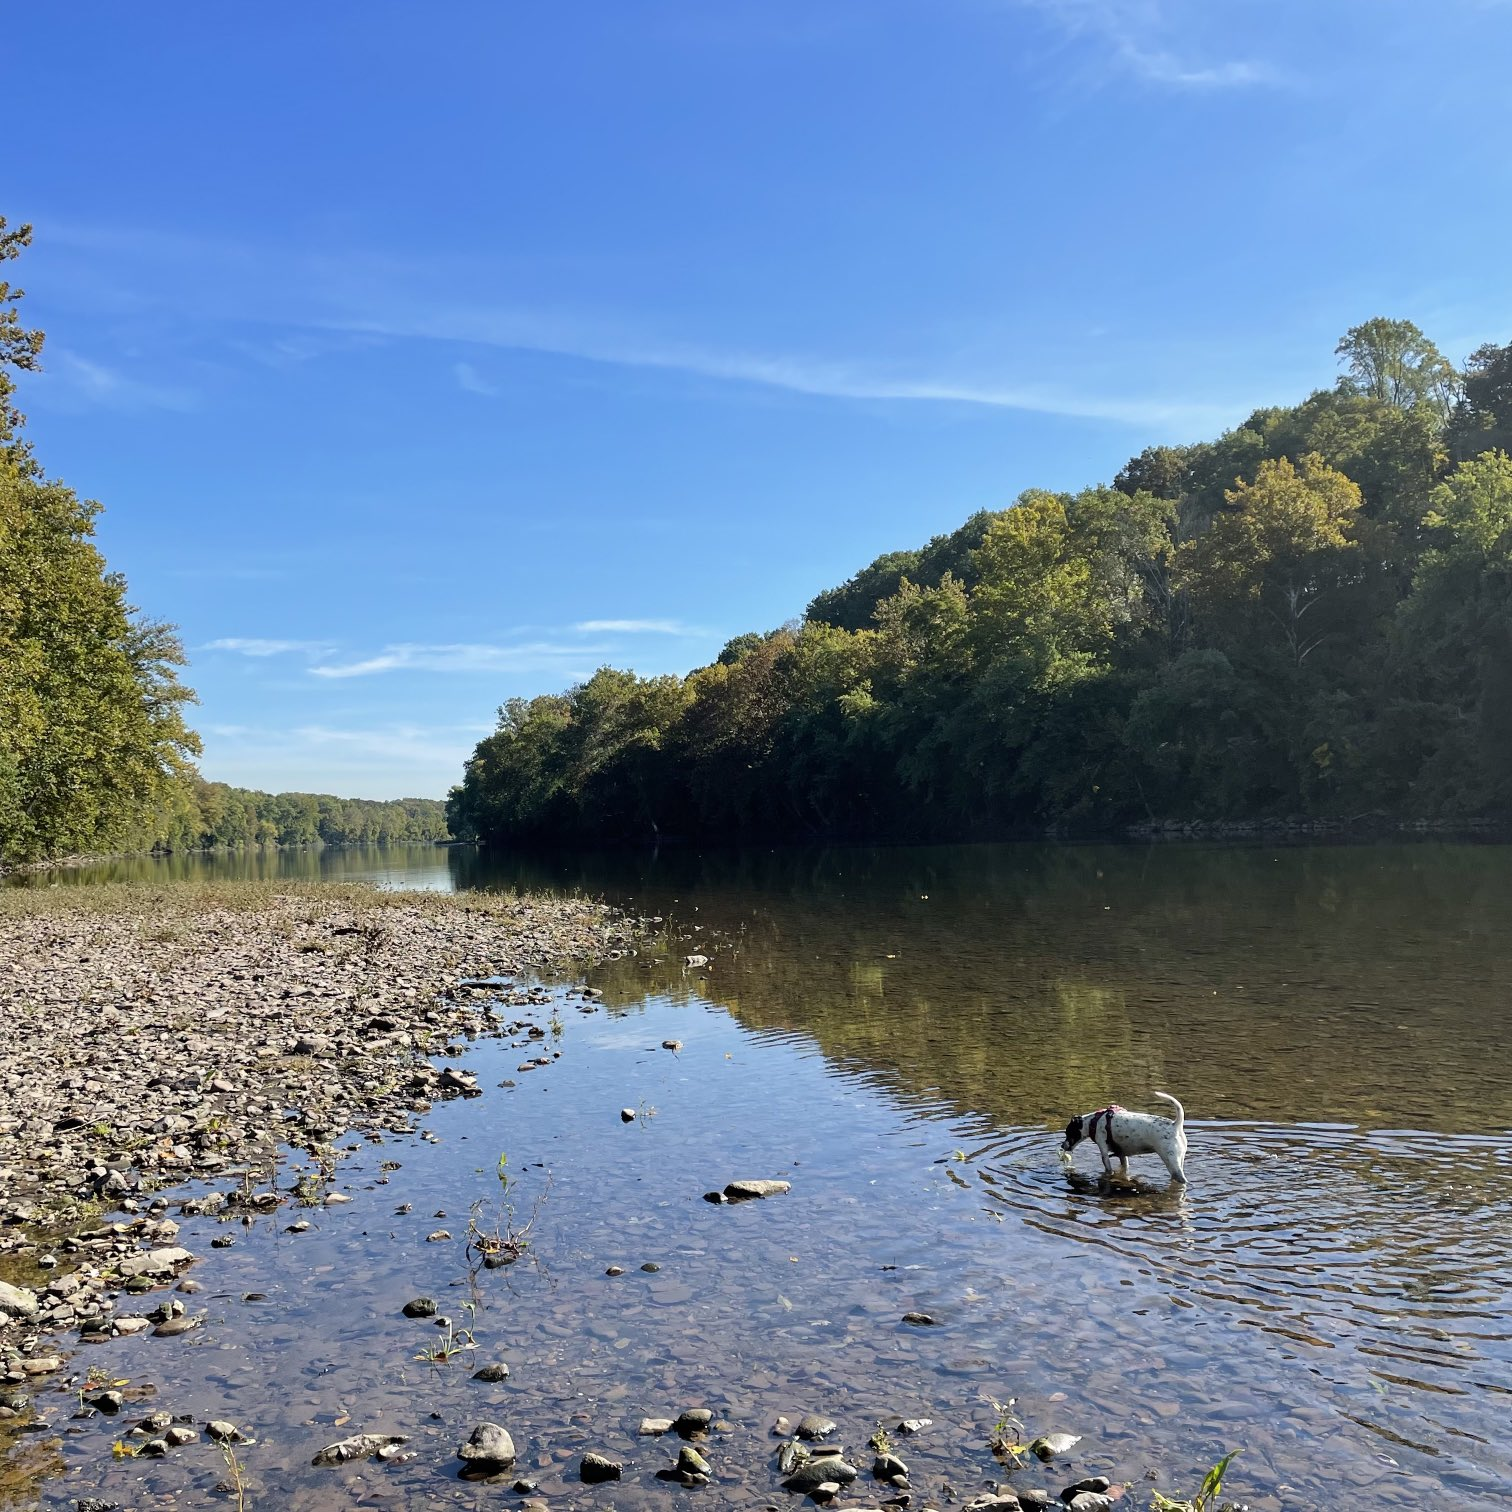
\includegraphics[width=0.75\linewidth]{./images/river_crossing} 

\end{columns}
\end{frame}

\begin{frame}{}
\protect\hypertarget{section-3}{}
\begin{itemize}
\tightlist
\item
  The mean is the preferred measure of central tendency when describing
  a data that do not have outliers.
\item
  A major disadvantage is that it is affected by outliers (i.e.~single
  observations which are very extreme compared with most observations
  and whose inclusion or exclusion changes results noticeably).
\item
  In the presence of outliers, the median is the preferred measure of
  central tendency
\item
  Calculation of the median does not involve the use of all available
  data and is therefore has less power than the mean.
\end{itemize}
\end{frame}

\begin{frame}{Partition values}
\protect\hypertarget{partition-values}{}
\begin{block}{Quartiles}

\small
A quartile is one of 4 values (lower quartile, median and upper quartile) which divides data into 4 equal groups.
\end{block}

\begin{block}{Percentiles}
\small
A percentile is one of 99 values which divides data into 100 equal groups. The lower quartile corresponds to the 25th percentile. The median corresponds to the 50th percentile and the upper quartile corresponds to the 75th percentile.

Formally, the percentile is:

$$
\text{Percentile (P)} = (1 - w)x_{(j)} + wx_{(j+1)}
$$
For some weight $w$ between 0 and 1. Different approaches to choosing $w$ are described -- In R, there are nine different alternatives to compute the quantile. 

\end{block}
\end{frame}

\begin{frame}{Geometric mean}
\protect\hypertarget{geometric-mean}{}
\small

In mathematics, geometric mean is a mean or average, which indicates the
central tendency or typical value of a set of numbers by using the
product of their values (as opposed to the arithmetic mean which uses
their sum). The geometric mean is defined as the \(n^{\text{th}}\) root
of the product of \(n\) numbers, i.e., for a set of numbers
\(x_1, x_2, x_3, ..., x_n\), the geometric mean is defined as:

\[
\left(\prod _{i=1}^{n}x_{i}\right)^{\frac {1}{n}}={\sqrt[{n}]{x_{1}x_{2}\cdots x_{n}}} = \exp\left(\frac{1}{n} \sum_{i = 1}^n \ln \alpha_i \right)
\]

For the example book sales data mentioned above (
\(0, 0, 0, 1, 5, 5, 5, 5, 5, 5, 6 , 7, 7, 8, 10, 10, 11, 12, 13, 14\)),
the geometric mean is (note the data contain 0 as values, logarithmic
transformation of which is undefined so adding a positive value before
the transformation and subtraction after exponentiation should give
proper geometric mean): 4.74.
\end{frame}

\begin{frame}{Relationship between GM, AM and HM}
\protect\hypertarget{relationship-between-gm-am-and-hm}{}
\begin{figure}
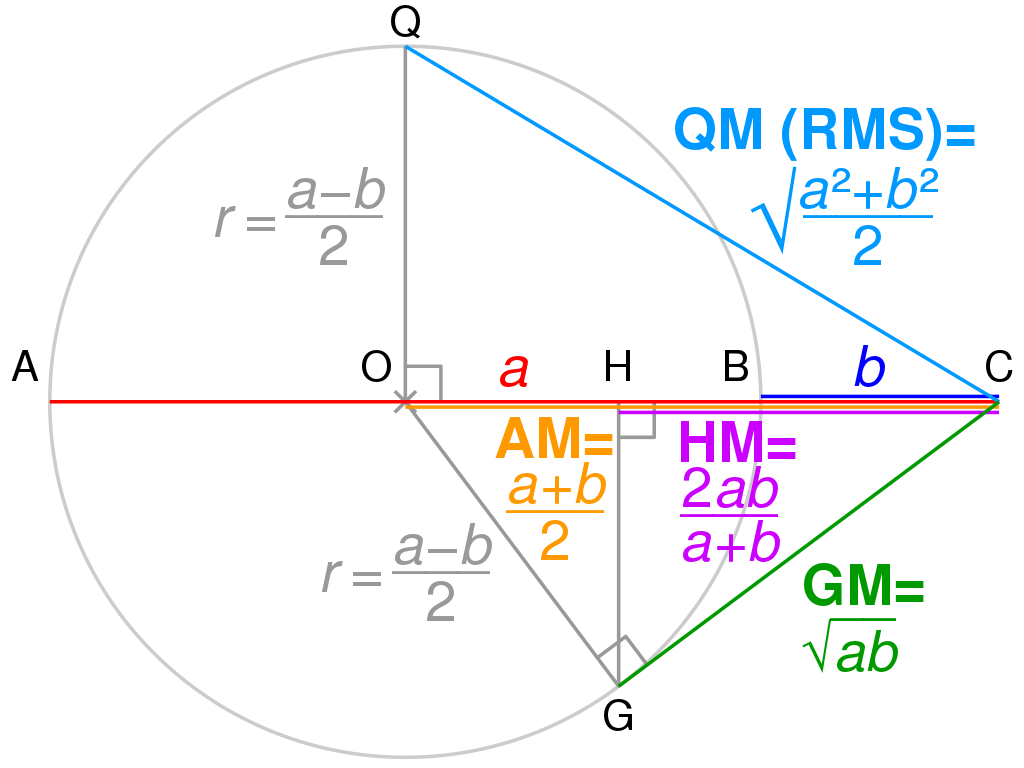
\includegraphics[width=0.45\linewidth]{./images/geometric_proof_hm_am_gm} \caption{Geometric proof that max(a,b) > root mean square (RMS) or quadratic mean (QM) > arithmetic mean (AM) > geometric mean (GM) > harmonic mean (HM) > min(a,b) of two distinct positive numbers a and b. \textit{Source:\url{https://en.wikipedia.org/wiki/Geometric_mean}}}\label{fig:inequality-relation-gm-am-hm}
\end{figure}
\end{frame}

\hypertarget{graphical-method-of-data-presentation}{%
\section{Graphical method of data
presentation}\label{graphical-method-of-data-presentation}}

\begin{frame}{Diagrammatic presentation of data}
\protect\hypertarget{diagrammatic-presentation-of-data}{}
\begin{itemize}
\tightlist
\item
  Bar

  \begin{itemize}
  \tightlist
  \item
    A graph of a frequency distribution for a categorical data set. Each
    category is represented by a segment of the bar, and the area of the
    segment is proportional to the corresponding frequency or relative
    frequency.
  \end{itemize}
\item
  Pie

  \begin{itemize}
  \tightlist
  \item
    A graph of a frequency distribution for a categorical data set. Each
    category is represented by a slice of the pie, and the area of the
    slice is proportional to the corresponding frequency or relative
    frequency.
  \end{itemize}
\item
  Histogram

  \begin{itemize}
  \tightlist
  \item
    A picture of the information in a frequency distribution for a
    numerical data set. A rectangle is drawn above each possible value
    (discretized data) or class interval. The rectangle's area is
    proportional to the corresponding frequency or relative frequency.
  \end{itemize}
\item
  Frequency polygon
\item
  Frequency curve
\item
  Ogives (cumulative frequency curves)
\end{itemize}
\end{frame}

\begin{frame}{Histogram}
\protect\hypertarget{histogram}{}
\begin{columns}[T, onlytextwidth]
\column{0.45\textwidth}
\begin{itemize}
\footnotesize
\item Histogram shows the shape of a distribution.
\item Distribution can be called unimodal (one peak), bimodal (two peaks) or multimodal (multiple peaks).
\item Distribution can be symmetric or skewed. A skewed distribution is asymmetrical with a longer tail on one side. \end{itemize}


\begin{center}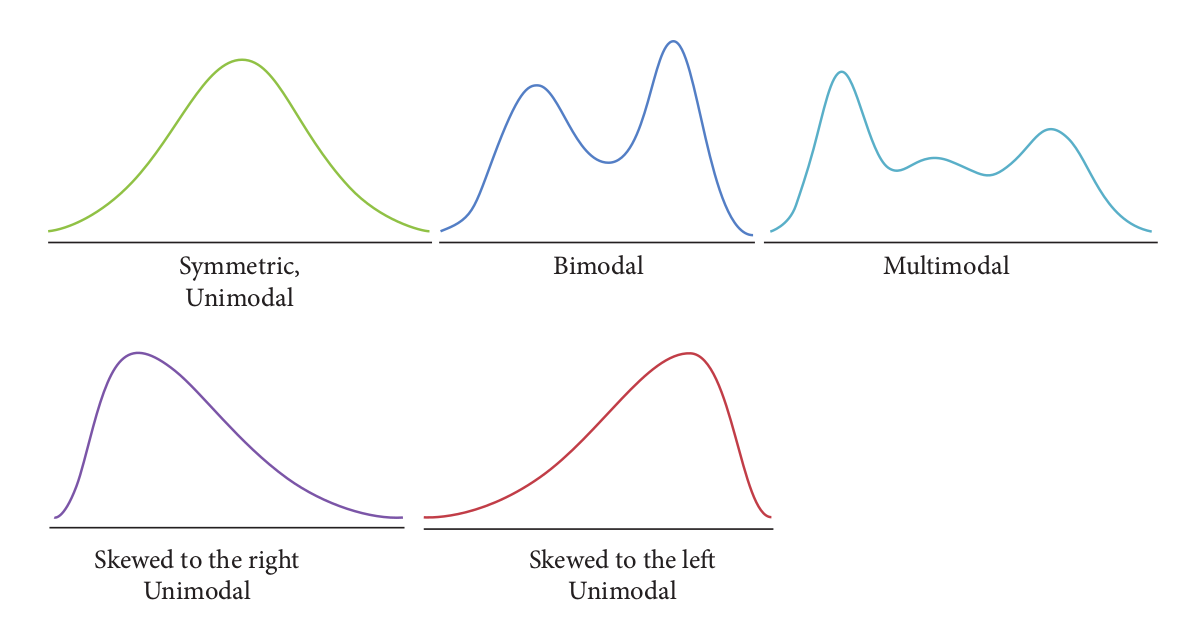
\includegraphics[width=0.8\linewidth]{./images/distribution_types} \end{center}

\column{0.55\textwidth}

\begin{itemize}
\footnotesize
\item Let us consider the marks in a subject obtained by 300 candidates selected at random among those appearing a certain examination.
\end{itemize}

\begin{table}
\centering\begingroup\fontsize{6}{8}\selectfont

\begin{tabular}{lr}
\toprule
Score class & Frequency\\
\midrule
(45.1,55.9] & 65\\
(55.9,66.6] & 58\\
(66.6,77.4] & 51\\
(77.4,88.1] & 66\\
(88.1,98.9] & 60\\
\bottomrule
\end{tabular}
\endgroup{}
\end{table}



\begin{center}\includegraphics[width=0.45\linewidth]{03.4-measures_of_central_tendency_frequency_distributions_files/figure-beamer/student-marks-hist-1} \end{center}

\end{columns}
\end{frame}

\begin{frame}{Bar diagram}
\protect\hypertarget{bar-diagram}{}
\begin{columns}[T, onlytextwidth]
\column{0.5\textwidth}

\begin{itemize}
\footnotesize
\item A bar diagram is a pictorial representation of a frequency distribution of categorical data.
\item It is Useful to represent data with multiple occurrence or counts.
\item Pie diagram accommodates lesser classes and better shows relative proportion of occurrences or count data.
\item For the table \ref{tab:midterm-frequency-dist}, we can generate a bar diagram as shown in \ref{fig:midterm-frequency-bar}.
\end{itemize}



\column{0.5\textwidth}

\begin{figure}
\includegraphics[width=0.5\linewidth]{03.4-measures_of_central_tendency_frequency_distributions_files/figure-beamer/midterm-frequency-bar-1} \caption{Bar graph showing frequency distribution of mid-term scores of 22 pupils}\label{fig:midterm-frequency-bar}
\end{figure}

\end{columns}

\begin{table}

\caption{\label{tab:midterm-frequency-dist}Frequency distribution of mid-term scores of 22 pupils in a statistics exam}
\centering
\fontsize{5}{7}\selectfont
\begin{tabular}[t]{>{\raggedright\arraybackslash}p{2em}>{\raggedright\arraybackslash}p{0.5em}>{\raggedright\arraybackslash}p{0.5em}>{\raggedright\arraybackslash}p{0.5em}>{\raggedright\arraybackslash}p{0.5em}>{\raggedright\arraybackslash}p{0.5em}>{\raggedright\arraybackslash}p{0.5em}>{\raggedright\arraybackslash}p{0.5em}>{\raggedright\arraybackslash}p{0.5em}>{\raggedright\arraybackslash}p{0.5em}>{\raggedright\arraybackslash}p{0.5em}>{\raggedright\arraybackslash}p{0.5em}>{\raggedright\arraybackslash}p{0.5em}>{\raggedright\arraybackslash}p{0.5em}>{\raggedright\arraybackslash}p{0.5em}>{\raggedright\arraybackslash}p{0.5em}>{\raggedright\arraybackslash}p{0.5em}>{\raggedright\arraybackslash}p{0.5em}>{\raggedright\arraybackslash}p{0.5em}>{\raggedright\arraybackslash}p{0.5em}>{\raggedright\arraybackslash}p{0.5em}>{\raggedright\arraybackslash}p{0.5em}>{\raggedright\arraybackslash}p{0.5em}}
\toprule
pupil & 1 & 2 & 3 & 4 & 5 & 6 & 7 & 8 & 9 & 10 & 11 & 12 & 13 & 14 & 15 & 16 & 17 & 18 & 19 & 20 & 21 & 22\\
\midrule
scores & 69 & 84 & 52 & 93 & 81 & 74 & 89 & 85 & 88 & 63 & 87 & 90 & 67 & 72 & 74 & 55 & 82 & 91 & 68 & 77 & 70 & 77\\
\bottomrule
\end{tabular}
\end{table}
\end{frame}

\begin{frame}{Frequency polygon and cumulative frequency curve (Ogive)}
\protect\hypertarget{frequency-polygon-and-cumulative-frequency-curve-ogive}{}
\begin{columns}[T, onlytextwidth]
\column{0.4\textwidth}

\textbf{Frequency polygon}

\begin{itemize}
\footnotesize
\item Frequency curve, relatively smooth frequency curves, unlike polygons, is for continuous data. For example assume the mid term score data in its original form as being continuous.
\end{itemize}


\includegraphics[width=0.9\linewidth]{03.4-measures_of_central_tendency_frequency_distributions_files/figure-beamer/frequency-polygon-1} 

\column{0.6\textwidth}

\textbf{Ogives (cumulative frequency curves)}

\begin{figure}
\includegraphics[width=0.55\linewidth]{03.4-measures_of_central_tendency_frequency_distributions_files/figure-beamer/cumulative-frequency-curve-1} \caption{Cumulative frequency curve fitted to the mid-term score distribution}\label{fig:cumulative-frequency-curve}
\end{figure}

\begin{itemize}
\scriptsize
\item In the discrete frequency distribution, above, height of the bar shows relative frequency of each class.
\item When we use the height as the relative frequency if the interval lengths are unequal, histogram may not appropriately display the frequency distribution.
\end{itemize}
\end{columns}
\end{frame}

\hypertarget{tabular-method-of-data-presentation}{%
\section{Tabular method of data
presentation}\label{tabular-method-of-data-presentation}}

\hypertarget{tabular-methods-of-data-presentation}{%
\section{Tabular methods of data
presentation}\label{tabular-methods-of-data-presentation}}

\begin{frame}{Frequency distribution}
\protect\hypertarget{frequency-distribution}{}
\footnotesize

When observations of either discrete or continuous nature are available
on a single characteristic of a large number of individuals, often it
becomes necessary to condense the data as far as possible without losing
any information. A \textbf{frequency distribution} is a table that
displays the frequency of observation in each interval in a sample. To
build a frequency distribution, we need the following steps.

\begin{enumerate}
\tightlist
\item
  Find the minimum and the maximum values in the dataset
\item
  Determine class intervals: intervals or cells of equal length that
  cover the range between the minimum and the maximum without
  overlapping. e.g., minimum 0, maximum 100: {[}0, 10), {[}10, 20),
  \ldots, {[}90, 100).
\item
  Find frequency: the number of observations in the data that belog to
  each class interval. Let's denote the frequencies as \(f_1, f_2, ...\)
\item
  Find relative frequency:
\end{enumerate}

\[
\frac{\textrm{Class frequency}}{\textrm{Total number of observations}}
\]

The relative frequency are denoted as \(f_1/n, f_2/n, ...\) if the total
sample size is n.
\end{frame}

\begin{frame}{}
\protect\hypertarget{section-4}{}
\begin{itemize}
\tightlist
\item
  For example, for the Mid-term scores data (Shown in Table
  \ref{tab:midterm-frequency-dist}), we could construct class intervals
  to show relative frequencies as follows:
\end{itemize}

\begin{table}

\caption{\label{tab:midterm-frequency-class-tab}Relative frequencies of mid-term scores expressed in score classes of interval 10}
\centering
\begin{tabular}[t]{lrl}
\toprule
Class interval & Frequency & Relative frequency\\
\midrule
50-59 & 2 & 9.1\%\\
60-69 & 4 & 18.2\%\\
70-79 & 6 & 27.3\%\\
80-89 & 7 & 31.8\%\\
90-99 & 3 & 13.6\%\\
\bottomrule
\end{tabular}
\end{table}

\begin{itemize}
\tightlist
\item
  There is no gold standard in selecting class intervals, but a rule of
  thumb is an integer near \(\sqrt n\) for the number of classes.
\end{itemize}
\end{frame}

\begin{frame}{}
\protect\hypertarget{section-5}{}
\begin{itemize}
\tightlist
\item
  Tabular data facilitates the presentation of large information into
  concise way under different titles and subtitles so that can further
  be subjected to statistical analysis.

  \begin{itemize}
  \tightlist
  \item
    Simple tabulation (for single variable; e.g., Table
    \ref{tab:midterm-frequency-class-tab})
  \item
    Double tabulation (tabulation of different crops under condition of
    irrigation and without irrigation)
  \item
    Triple tabulation
  \item
    Manifold tabulation (Tabulation based on more than 3
    characteristics; data of students in a college according to native
    place, class residence and sex.)
  \end{itemize}
\end{itemize}
\end{frame}

\begin{frame}{}
\protect\hypertarget{section-6}{}
\begin{columns}[T, onlytextwidth]
\column{0.5\textwidth}

\begin{table}
\centering\begingroup\fontsize{7}{9}\selectfont

\begin{tabular}{llllr}
\toprule
 &  & Residence & Class & n\\
\midrule
\addlinespace[0.3em]
\multicolumn{5}{l}{\textbf{Rural}}\\
\addlinespace[0.3em]
\multicolumn{5}{l}{\textit{Female}}\\
\hspace{1em}\hspace{1em} &  & Hostellers & Graduate & 13\\
\cmidrule{4-5}
\hspace{1em}\hspace{1em}\hspace{1em}\hspace{1em} &  &  & Intermediate & 7\\
\cmidrule{4-5}
\hspace{1em}\hspace{1em} &  &  & Post Graduate & 7\\
\cmidrule{3-5}
\hspace{1em}\hspace{1em} &  & Scholars & Graduate & 20\\
\cmidrule{4-5}
\hspace{1em}\hspace{1em}\hspace{1em}\hspace{1em} &  &  & Intermediate & 3\\
\cmidrule{4-5}
\hspace{1em}\hspace{1em} &  &  & Post Graduate & 13\\
\cmidrule{2-5}
\addlinespace[0.3em]
\multicolumn{5}{l}{\textit{Male}}\\
\hspace{1em}\hspace{1em} &  & Hostellers & Graduate & 16\\
\cmidrule{4-5}
 &  &  & Intermediate & 3\\
\cmidrule{4-5}
\hspace{1em}\hspace{1em} &  &  & Post Graduate & 6\\
\cmidrule{3-5}
\hspace{1em}\hspace{1em} &  & Scholars & Graduate & 13\\
\cmidrule{4-5}
 &  &  & Intermediate & 7\\
\cmidrule{4-5}
\hspace{1em}\hspace{1em} &  &  & Post Graduate & 22\\
\bottomrule
\end{tabular}
\endgroup{}
\end{table}

\column{0.5\textwidth}

\begin{table}
\centering\begingroup\fontsize{7}{9}\selectfont

\begin{tabular}{llllr}
\toprule
 &  & Residence & Class & n\\
\midrule
\addlinespace[0.3em]
\multicolumn{5}{l}{\textbf{Urban}}\\
\addlinespace[0.3em]
\multicolumn{5}{l}{\textit{Female}}\\
\hspace{1em}\hspace{1em} &  & Hostellers & Graduate & 2\\
\cmidrule{4-5}
\hspace{1em}\hspace{1em}\hspace{1em}\hspace{1em} &  &  & Intermediate & 2\\
\cmidrule{4-5}
\hspace{1em}\hspace{1em}\hspace{1em}\hspace{1em} &  &  & Post Graduate & 2\\
\cmidrule{3-5}
\hspace{1em}\hspace{1em} &  & Scholars & Graduate & 3\\
\cmidrule{4-5}
\hspace{1em}\hspace{1em} &  &  & Intermediate & 4\\
\cmidrule{4-5}
 &  &  & Post Graduate & 2\\
\cmidrule{2-5}
\addlinespace[0.3em]
\multicolumn{5}{l}{\textit{Male}}\\
\hspace{1em}\hspace{1em} &  & Hostellers & Graduate & 4\\
\cmidrule{4-5}
\hspace{1em}\hspace{1em} &  &  & Intermediate & 1\\
\cmidrule{4-5}
\hspace{1em}\hspace{1em} &  &  & Post Graduate & 1\\
\cmidrule{3-5}
\hspace{1em}\hspace{1em} &  & Scholars & Graduate & 6\\
\cmidrule{4-5}
 &  &  & Intermediate & 2\\
\bottomrule
\end{tabular}
\endgroup{}
\end{table}

\end{columns}
\end{frame}

\begin{frame}{Question 1}
\protect\hypertarget{question-1}{}
A group of 50 biomedical students recorded their pulse rates by counting
the number of beats for 30 seconds and multiplying by 2.

\begin{enumerate}
[a.]
\tightlist
\item
  Why are all of the measurements even number ?
\item
  Draw a stem and leaf plot to describe the data, splitting each stem
  into two lines.
\item
  Construct a relative frequency histogram for the data.
\item
  Write a short paragraph describing the distribution of the student
  pulse rates.
\end{enumerate}
\end{frame}

\begin{frame}[fragile]{Solution 1}
\protect\hypertarget{solution-1}{}
\begin{enumerate}
[a.]
\item
  Because the resulting data is constructed from multiplication of
  original values by an even integer.
\item
  Stem and leaf plot is:
\end{enumerate}

\begin{verbatim}
## 
##   The decimal point is 1 digit(s) to the right of the |
## 
##    4 | 2
##    5 | 24688
##    6 | 002266668
##    7 | 0002222248
##    8 | 002244444444468888
##    9 | 0066
##   10 | 04
##   11 | 0
\end{verbatim}

\begin{enumerate}
[a.]
\setcounter{enumi}{2}
\tightlist
\item
  Relative frequency histogram for data:
\end{enumerate}

\includegraphics[width=0.45\linewidth]{03.4-measures_of_central_tendency_frequency_distributions_files/figure-beamer/unnamed-chunk-4-1}

The distribution is skewed to right because distribution presents long
left tail.
\end{frame}

\end{document}
